% Options for packages loaded elsewhere
% Options for packages loaded elsewhere
\PassOptionsToPackage{unicode}{hyperref}
\PassOptionsToPackage{hyphens}{url}
%
\documentclass[
  ignorenonframetext,
  aspectratio=169,
]{beamer}
\newif\ifbibliography
\usepackage{pgfpages}
\setbeamertemplate{caption}[numbered]
\setbeamertemplate{caption label separator}{: }
\setbeamercolor{caption name}{fg=normal text.fg}
\beamertemplatenavigationsymbolsempty
% remove section numbering
\setbeamertemplate{part page}{
  \centering
  \begin{beamercolorbox}[sep=16pt,center]{part title}
    \usebeamerfont{part title}\insertpart\par
  \end{beamercolorbox}
}
\setbeamertemplate{section page}{
  \centering
  \begin{beamercolorbox}[sep=12pt,center]{section title}
    \usebeamerfont{section title}\insertsection\par
  \end{beamercolorbox}
}
\setbeamertemplate{subsection page}{
  \centering
  \begin{beamercolorbox}[sep=8pt,center]{subsection title}
    \usebeamerfont{subsection title}\insertsubsection\par
  \end{beamercolorbox}
}
% Prevent slide breaks in the middle of a paragraph
\widowpenalties 1 10000
\raggedbottom
\AtBeginPart{
  \frame{\partpage}
}
\AtBeginSection{
  \ifbibliography
  \else
    \frame{\sectionpage}
  \fi
}
\AtBeginSubsection{
  \frame{\subsectionpage}
}
\usepackage{iftex}
\ifPDFTeX
  \usepackage[T1]{fontenc}
  \usepackage[utf8]{inputenc}
  \usepackage{textcomp} % provide euro and other symbols
\else % if luatex or xetex
  \usepackage{unicode-math} % this also loads fontspec
  \defaultfontfeatures{Scale=MatchLowercase}
  \defaultfontfeatures[\rmfamily]{Ligatures=TeX,Scale=1}
\fi
\usepackage{lmodern}

\usetheme[]{Boadilla}
\usecolortheme[]{default}
\usefonttheme[]{professionalfonts}
\ifPDFTeX\else
  % xetex/luatex font selection
\fi
% Use upquote if available, for straight quotes in verbatim environments
\IfFileExists{upquote.sty}{\usepackage{upquote}}{}
\IfFileExists{microtype.sty}{% use microtype if available
  \usepackage[]{microtype}
  \UseMicrotypeSet[protrusion]{basicmath} % disable protrusion for tt fonts
}{}
\makeatletter
\@ifundefined{KOMAClassName}{% if non-KOMA class
  \IfFileExists{parskip.sty}{%
    \usepackage{parskip}
  }{% else
    \setlength{\parindent}{0pt}
    \setlength{\parskip}{6pt plus 2pt minus 1pt}}
}{% if KOMA class
  \KOMAoptions{parskip=half}}
\makeatother

\usepackage{color}
\usepackage{fancyvrb}
\newcommand{\VerbBar}{|}
\newcommand{\VERB}{\Verb[commandchars=\\\{\}]}
\DefineVerbatimEnvironment{Highlighting}{Verbatim}{commandchars=\\\{\}}
% Add ',fontsize=\small' for more characters per line
\usepackage{framed}
\definecolor{shadecolor}{RGB}{241,243,245}
\newenvironment{Shaded}{\begin{snugshade}}{\end{snugshade}}
\newcommand{\AlertTok}[1]{\textcolor[rgb]{0.68,0.00,0.00}{#1}}
\newcommand{\AnnotationTok}[1]{\textcolor[rgb]{0.37,0.37,0.37}{#1}}
\newcommand{\AttributeTok}[1]{\textcolor[rgb]{0.40,0.45,0.13}{#1}}
\newcommand{\BaseNTok}[1]{\textcolor[rgb]{0.68,0.00,0.00}{#1}}
\newcommand{\BuiltInTok}[1]{\textcolor[rgb]{0.00,0.23,0.31}{#1}}
\newcommand{\CharTok}[1]{\textcolor[rgb]{0.13,0.47,0.30}{#1}}
\newcommand{\CommentTok}[1]{\textcolor[rgb]{0.37,0.37,0.37}{#1}}
\newcommand{\CommentVarTok}[1]{\textcolor[rgb]{0.37,0.37,0.37}{\textit{#1}}}
\newcommand{\ConstantTok}[1]{\textcolor[rgb]{0.56,0.35,0.01}{#1}}
\newcommand{\ControlFlowTok}[1]{\textcolor[rgb]{0.00,0.23,0.31}{\textbf{#1}}}
\newcommand{\DataTypeTok}[1]{\textcolor[rgb]{0.68,0.00,0.00}{#1}}
\newcommand{\DecValTok}[1]{\textcolor[rgb]{0.68,0.00,0.00}{#1}}
\newcommand{\DocumentationTok}[1]{\textcolor[rgb]{0.37,0.37,0.37}{\textit{#1}}}
\newcommand{\ErrorTok}[1]{\textcolor[rgb]{0.68,0.00,0.00}{#1}}
\newcommand{\ExtensionTok}[1]{\textcolor[rgb]{0.00,0.23,0.31}{#1}}
\newcommand{\FloatTok}[1]{\textcolor[rgb]{0.68,0.00,0.00}{#1}}
\newcommand{\FunctionTok}[1]{\textcolor[rgb]{0.28,0.35,0.67}{#1}}
\newcommand{\ImportTok}[1]{\textcolor[rgb]{0.00,0.46,0.62}{#1}}
\newcommand{\InformationTok}[1]{\textcolor[rgb]{0.37,0.37,0.37}{#1}}
\newcommand{\KeywordTok}[1]{\textcolor[rgb]{0.00,0.23,0.31}{\textbf{#1}}}
\newcommand{\NormalTok}[1]{\textcolor[rgb]{0.00,0.23,0.31}{#1}}
\newcommand{\OperatorTok}[1]{\textcolor[rgb]{0.37,0.37,0.37}{#1}}
\newcommand{\OtherTok}[1]{\textcolor[rgb]{0.00,0.23,0.31}{#1}}
\newcommand{\PreprocessorTok}[1]{\textcolor[rgb]{0.68,0.00,0.00}{#1}}
\newcommand{\RegionMarkerTok}[1]{\textcolor[rgb]{0.00,0.23,0.31}{#1}}
\newcommand{\SpecialCharTok}[1]{\textcolor[rgb]{0.37,0.37,0.37}{#1}}
\newcommand{\SpecialStringTok}[1]{\textcolor[rgb]{0.13,0.47,0.30}{#1}}
\newcommand{\StringTok}[1]{\textcolor[rgb]{0.13,0.47,0.30}{#1}}
\newcommand{\VariableTok}[1]{\textcolor[rgb]{0.07,0.07,0.07}{#1}}
\newcommand{\VerbatimStringTok}[1]{\textcolor[rgb]{0.13,0.47,0.30}{#1}}
\newcommand{\WarningTok}[1]{\textcolor[rgb]{0.37,0.37,0.37}{\textit{#1}}}

\usepackage{longtable,booktabs,array}
\newcounter{none} % for unnumbered tables
\usepackage{calc} % for calculating minipage widths
\usepackage{caption}
% Make caption package work with longtable
\makeatletter
\def\fnum@table{\tablename~\thetable}
\makeatother
\usepackage{graphicx}
\makeatletter
\newsavebox\pandoc@box
\newcommand*\pandocbounded[1]{% scales image to fit in text height/width
  \sbox\pandoc@box{#1}%
  \Gscale@div\@tempa{\textheight}{\dimexpr\ht\pandoc@box+\dp\pandoc@box\relax}%
  \Gscale@div\@tempb{\linewidth}{\wd\pandoc@box}%
  \ifdim\@tempb\p@<\@tempa\p@\let\@tempa\@tempb\fi% select the smaller of both
  \ifdim\@tempa\p@<\p@\scalebox{\@tempa}{\usebox\pandoc@box}%
  \else\usebox{\pandoc@box}%
  \fi%
}
% Set default figure placement to htbp
\def\fps@figure{htbp}
\makeatother





\setlength{\emergencystretch}{3em} % prevent overfull lines

\providecommand{\tightlist}{%
  \setlength{\itemsep}{0pt}\setlength{\parskip}{0pt}}



 


\makeatletter
\@ifpackageloaded{caption}{}{\usepackage{caption}}
\AtBeginDocument{%
\ifdefined\contentsname
  \renewcommand*\contentsname{Table of contents}
\else
  \newcommand\contentsname{Table of contents}
\fi
\ifdefined\listfigurename
  \renewcommand*\listfigurename{List of Figures}
\else
  \newcommand\listfigurename{List of Figures}
\fi
\ifdefined\listtablename
  \renewcommand*\listtablename{List of Tables}
\else
  \newcommand\listtablename{List of Tables}
\fi
\ifdefined\figurename
  \renewcommand*\figurename{Figure}
\else
  \newcommand\figurename{Figure}
\fi
\ifdefined\tablename
  \renewcommand*\tablename{Table}
\else
  \newcommand\tablename{Table}
\fi
}
\@ifpackageloaded{float}{}{\usepackage{float}}
\floatstyle{ruled}
\@ifundefined{c@chapter}{\newfloat{codelisting}{h}{lop}}{\newfloat{codelisting}{h}{lop}[chapter]}
\floatname{codelisting}{Listing}
\newcommand*\listoflistings{\listof{codelisting}{List of Listings}}
\makeatother
\makeatletter
\makeatother
\makeatletter
\@ifpackageloaded{caption}{}{\usepackage{caption}}
\@ifpackageloaded{subcaption}{}{\usepackage{subcaption}}
\makeatother

\usepackage{bookmark}
\IfFileExists{xurl.sty}{\usepackage{xurl}}{} % add URL line breaks if available
\urlstyle{same}
\hypersetup{
  pdftitle={Lecture 3: Poisson Processes},
  hidelinks,
  pdfcreator={LaTeX via pandoc}}


\title{\texorpdfstring{Lecture 3: Poisson
Processes}{Lecture 3: Poisson Processes}}
\author{}
\date{}

\begin{document}
\frame{\titlepage}


\section{Introduction to Poisson
Processes}\label{introduction-to-poisson-processes}

\begin{frame}{Motivation}
\protect\phantomsection\label{motivation}
Many real-world systems involve events occurring over time. Examples
include insurance claims, customer arrivals, and financial transactions.

In previous chapters, we studied Markov chains, which describe systems
that evolve through a sequence of discrete time steps. We now consider
stochastic processes in which events can occur at any time in a
continuous time interval.

Poisson processes provide a mathematical model for counting such events
and studying when they occur.
\end{frame}

\begin{frame}{From Markov Chains to Poisson Processes}
\protect\phantomsection\label{from-markov-chains-to-poisson-processes}
A discrete-time Markov chain describes the evolution of a system at
times \(n=0,1,2,\ldots\). Its future state depends on the current state,
given the past.

A Poisson process instead tracks the number of events that have occurred
by time \(t\), where \(t\geq 0\) is continuous.

The distinction is that a Poisson process models event arrivals over
continuous time. Although the Poisson process is itself a Markov
process, its time parameter is continuous rather than discrete.
\end{frame}

\begin{frame}{Counting Events over Time}
\protect\phantomsection\label{counting-events-over-time}
Let \(N(t)\) denote the number of events that occur during the time
interval \((0,t]\). The collection \(\{N(t):t\geq 0\}\) is called a
counting process.

The process starts at \(N(0)=0\) and is non-decreasing: if
\(0\leq s\leq t\), then \(N(s)\leq N(t)\).

For example, if three claims occur by time \(t=5\), then \(N(5)=3\). If
two more claims occur between times \(5\) and \(8\), then \(N(8)=5\).
\end{frame}

\begin{frame}{Applications}
\protect\phantomsection\label{applications}
Poisson processes are used to model event arrivals in many fields.

\begin{itemize}
\tightlist
\item
  \textbf{Insurance:} the number of claims reported to an insurer over
  time.
\item
  \textbf{Finance:} the arrival of credit defaults or certain types of
  financial events.
\item
  \textbf{Telecommunications:} the number of calls received by a call
  centre.
\item
  \textbf{Transportation:} the number of accidents occurring on a
  highway.
\item
  \textbf{Healthcare:} the number of patients arriving at an emergency
  department.
\end{itemize}

The suitability of the model depends on whether its assumptions
reasonably describe the event-generating mechanism.
\end{frame}

\begin{frame}{Questions of Interest}
\protect\phantomsection\label{questions-of-interest}
Suppose insurance claims arrive at an average rate of \(\lambda=20\)
claims per day.

We may ask:

\begin{itemize}
\tightlist
\item
  What is the probability that more than 100 claims arrive during a
  seven-day period?
\item
  What is the expected waiting time until the next claim?
\item
  What is the probability that no claims occur during the next two
  hours?
\end{itemize}

A Poisson process provides a framework for answering these questions by
modelling both the number of events and the time between successive
events.
\end{frame}

\begin{frame}{Assumptions Underlying the Poisson Process}
\protect\phantomsection\label{assumptions-underlying-the-poisson-process}
A homogeneous Poisson process with rate \(\lambda>0\) is based on the
following assumptions.

\begin{itemize}
\tightlist
\item
  \textbf{Independent increments:} the numbers of events occurring in
  disjoint time intervals are independent.
\item
  \textbf{Stationary increments:} the distribution of the number of
  events in an interval depends only on the interval's length, not on
  its starting time.
\item
  \textbf{Constant rate:} the expected number of events in an interval
  of length \(t\) is \(\lambda t\).
\item
  \textbf{Negligible probability of multiple events in a very short
  interval:} over a small interval of length \(h\), the probability of
  two or more events is of smaller order than \(h\).
\end{itemize}

The parameter \(\lambda\) is the average number of events per unit time.
It must be measured using a consistent time unit.

These assumptions lead to the Poisson distribution for event counts and
the exponential distribution for interarrival times, which will be
developed in the following sections.
\end{frame}

\section{The Poisson Process}\label{the-poisson-process}

\begin{frame}{Definition and Notation}
\protect\phantomsection\label{definition-and-notation}
A Poisson process is a counting process \(\{N(t):t\geq 0\}\) that models
the number of events occurring over time.

\begin{itemize}
\tightlist
\item
  \(N(0)=0\), and \(N(t)\) is a non-negative integer.
\item
  \(N(t)\) is non-decreasing and has a right-continuous step-function
  sample path.
\item
  For \(0\leq s<t\), the number of events in \((s,t]\) is \(N(t)-N(s)\).
\end{itemize}

A homogeneous Poisson process with rate \(\lambda>0\) has independent
increments, stationary increments, and an event rate that is constant
over time.
\end{frame}

\begin{frame}{Homogeneous Poisson Process}
\protect\phantomsection\label{homogeneous-poisson-process}
A homogeneous Poisson process models the number of events occurring
randomly over time at a constant average rate.

Examples include insurance claims, customer arrivals, and equipment
failures.

A counting process \(\{N(t):t\geq 0\}\) is a homogeneous Poisson process
with rate \(\lambda>0\) if it satisfies:

\begin{itemize}
\tightlist
\item
  \textbf{Initial condition:} \(N(0)=0\).
\item
  \textbf{Independent increments:} Event counts in disjoint time
  intervals are independent.
\item
  \textbf{Stationary increments:} The distribution of the event count
  depends only on the interval length.
\item
  \textbf{Poisson distribution:} For \(s,t\geq 0\), \[
  N(s+t)-N(s)\sim\operatorname{Poisson}(\lambda t).
  \]
\end{itemize}

Here, \(\lambda\) is the constant average number of events per unit
time.
\end{frame}

\begin{frame}{The Poisson Distribution of Event Counts}
\protect\phantomsection\label{the-poisson-distribution-of-event-counts}
For a homogeneous Poisson process with rate \(\lambda\), the number of
events during an interval of length \(t\) follows a Poisson distribution
with parameter \(\lambda t\).

\[
N(t)\sim\operatorname{Poisson}(\lambda t).
\]

Hence, for \(n=0,1,2,\ldots\),

\[
\Pr(N(t)=n)=
\frac{(\lambda t)^n e^{-\lambda t}}{n!}.
\]

The mean and variance are both \(\lambda t\):

\[
\operatorname{E}[N(t)]=\operatorname{Var}[N(t)]=\lambda t.
\]
\end{frame}

\begin{frame}{The Rate Parameter}
\protect\phantomsection\label{the-rate-parameter}
The parameter \(\lambda\) is the constant event rate, measured as the
expected number of events per unit time.

For example, if an insurer receives an average of 20 claims per day,
then \(\lambda=20\) claims per day. Over a period of \(t\) days, the
expected number of claims is \(20t\).

The rate parameter determines how quickly events occur on average. A
larger \(\lambda\) means more events are expected over the same time
interval.

The rate is an average, not a guarantee that exactly \(\lambda t\)
events will occur.
\end{frame}

\begin{frame}{The Probability of No Events}
\protect\phantomsection\label{the-probability-of-no-events}
The probability of observing no events during an interval of length
\(t\) is obtained by setting \(n=0\) in the Poisson probability formula.

\[
\Pr(N(t)=0)=e^{-\lambda t}.
\]

By stationary increments, the same result applies to any interval
\((s,s+t]\):

\[
\Pr(N(s+t)-N(s)=0)=e^{-\lambda t}.
\]

For example, if claims arrive at a rate of \(\lambda=20\) per day, the
probability of no claims during the next hour is \(e^{-20/24}\),
assuming a day contains 24 hours.

The probability of no events decreases as either the event rate or the
length of the observation interval increases.
\end{frame}

\section{Definition and Properties of the Poisson
Process}\label{definition-and-properties-of-the-poisson-process}

\begin{frame}{The Poisson Process: Two Approaches}
\protect\phantomsection\label{the-poisson-process-two-approaches}
\begin{itemize}
\tightlist
\item
  A Poisson process models the occurrence of events over time, such as
  insurance claims or equipment failures.
\item
  Let \(N(t)\) denote the number of events occurring by time \(t\), with
  \(N(0)=0\).
\item
  The process has a constant rate \(\lambda>0\), measured in events per
  unit time.
\item
  There are two complementary ways to define a Poisson process:

  \begin{itemize}
  \tightlist
  \item
    \textbf{Local approach:} Describe the probabilities of events over a
    very short time interval.
  \item
    \textbf{Distributional approach:} Specify the distribution of event
    counts and the properties of increments.
  \end{itemize}
\item
  Both approaches describe the same homogeneous Poisson process under
  the appropriate assumptions.
\end{itemize}
\end{frame}

\begin{frame}{Definition 1: Local Behaviour}
\protect\phantomsection\label{definition-1-local-behaviour}
A counting process \(\{N(t):t\geq0\}\) is a Poisson process with rate
\(\lambda>0\) if it has independent increments and, as \(h\to0\),

\[
\begin{aligned}
\Pr(N(t+h)-N(t)=1)&=\lambda h+o(h),\\
\Pr(N(t+h)-N(t)=0)&=1-\lambda h+o(h),\\
\Pr(N(t+h)-N(t)\geq2)&=o(h).
\end{aligned}
\]

\begin{itemize}
\tightlist
\item
  The probability of one event in a short interval of length \(h\) is
  approximately \(\lambda h\).
\item
  The probability of two or more events is negligible relative to \(h\).
\item
  The notation \(o(h)\) means that \(o(h)/h\to0\) as \(h\to0\).
\item
  Independent increments mean that event counts in disjoint intervals
  are independent.
\end{itemize}
\end{frame}

\begin{frame}{Definition 1: Interpretation}
\protect\phantomsection\label{definition-1-interpretation}
\begin{itemize}
\tightlist
\item
  The rate \(\lambda\) is the average number of events per unit time.
\item
  For example, if claims arrive at an average rate of \(20\) per day,
  then \(\lambda=20\) claims per day.
\item
  Over a short interval of length \(h\) days, the probability of one
  claim is approximately \(20h\).
\item
  The approximation applies when \(h\) is sufficiently small.
\item
  The local conditions describe how events occur over short intervals;
  they do not directly give the distribution of the total number of
  events over a longer interval.
\end{itemize}
\end{frame}

\begin{frame}{Definition 2: Distributional Properties}
\protect\phantomsection\label{definition-2-distributional-properties}
A counting process \(\{N(t):t\geq0\}\) is a homogeneous Poisson process
with rate \(\lambda>0\) if:

\begin{itemize}
\item
  \(N(0)=0\).
\item
  It has independent increments.
\item
  For every \(0\leq s<t\),

  \[
  N(t)-N(s)\sim\operatorname{Poisson}(\lambda(t-s)).
  \]
\end{itemize}

Equivalently,

\[
\Pr(N(t)-N(s)=n)
=\frac{e^{-\lambda(t-s)}[\lambda(t-s)]^n}{n!},
\quad n=0,1,2,\ldots.
\]

\begin{itemize}
\tightlist
\item
  The increment distribution depends only on the interval length
  \(t-s\), so the process has stationary increments.
\end{itemize}
\end{frame}

\begin{frame}{Definition 2: Consequences}
\protect\phantomsection\label{definition-2-consequences}
Taking \(s=0\) gives

\[
N(t)\sim\operatorname{Poisson}(\lambda t).
\]

Hence, \(\operatorname{E}[N(t)]=\operatorname{Var}(N(t))=\lambda t.\)

The probability of no events in an interval of length \(t\) is

\[
\Pr(N(t)=0)=e^{-\lambda t}.
\]

The probability of at least one event is

\[
\Pr(N(t)\geq1)=1-e^{-\lambda t}.
\]

These results are useful for calculating event probabilities over
specified time intervals.
\end{frame}

\begin{frame}{How Are the Two Definitions Related?}
\protect\phantomsection\label{how-are-the-two-definitions-related}
\begin{itemize}
\tightlist
\item
  Definition 1 describes the local behaviour of the process.
\item
  Definition 2 describes the distribution of event counts over finite
  intervals.
\item
  Under the usual assumptions for a counting process, Definition 1,
  together with independent increments and \(N(0)=0\), leads to the
  Poisson distribution in Definition 2.
\item
  Conversely, the Poisson increment distribution implies the local
  probability conditions in Definition 1.
\end{itemize}

For example, if \(N(t)\) is a homogeneous Poisson process, then

\[
\begin{aligned}
\Pr(N(t+h)-N(t)=1)
&=e^{-\lambda h}\lambda h\\
&=\lambda h+o(h).
\end{aligned}
\]

Thus, the two approaches describe the same process, but emphasise
different properties.
\end{frame}

\begin{frame}{Which Definition Should We Use?}
\protect\phantomsection\label{which-definition-should-we-use}
\begin{itemize}
\tightlist
\item
  \textbf{Definition 1} explains the assumptions about event occurrences
  over short time intervals.
\item
  \textbf{Definition 2} is more convenient for calculating probabilities
  and deriving moments.
\item
  Both are useful: the local approach motivates the model, while the
  distributional approach supports most subsequent calculations.
\item
  In the following section, we use the Poisson process to study the
  times between successive events.
\end{itemize}
\end{frame}

\begin{frame}{Worked Example 1: Distribution of a Poisson Process}
\protect\phantomsection\label{worked-example-1-distribution-of-a-poisson-process}
Show that \(N(t)\) has a Poisson distribution with mean \(\lambda t\),
i.e.~\(N(t)\sim\operatorname{Poisson}(\lambda t)\).
\end{frame}

\begin{frame}{Solution: Worked Example 1}
\protect\phantomsection\label{solution-worked-example-1}
\end{frame}

\begin{frame}{Worked Example 2: Machinery Failures}
\protect\phantomsection\label{worked-example-2-machinery-failures}
Machinery failures at a factory occur according to a Poisson process
with a rate of one failure every eight hours. Calculate the probability
of one or more failures during a given hour.
\end{frame}

\begin{frame}{Solution: Worked Example 2}
\protect\phantomsection\label{solution-worked-example-2}
\end{frame}

\begin{frame}{Worked Example 3: Customer Arrivals}
\protect\phantomsection\label{worked-example-3-customer-arrivals}
Customers arrive at a coffee shop according to a Poisson process with a
rate of 10 customers per hour, starting at 9 a.m.

\begin{enumerate}
\tightlist
\item
  Calculate the probability that more than 30 customers arrive between
  11 a.m. and 1 p.m.
\item
  Calculate the probability that exactly 30 customers have arrived by
  noon and exactly 50 by 2 p.m.
\end{enumerate}
\end{frame}

\begin{frame}{Solution: Worked Example 3}
\protect\phantomsection\label{solution-worked-example-3}
\end{frame}

\begin{frame}{Worked Example 4: Independent Increments}
\protect\phantomsection\label{worked-example-4-independent-increments}
Let \(N(t)\) be a Poisson process with rate \(\lambda=5\) events per
hour.

\begin{enumerate}
\tightlist
\item
  Find the probability that exactly 3 events occur between 10 a.m. and
  11 a.m.
\item
  Find the probability that exactly 3 events occur between 10 a.m. and
  11 a.m. and exactly 4 events occur between 11 a.m. and noon.
\end{enumerate}
\end{frame}

\begin{frame}{Solution: Worked Example 4}
\protect\phantomsection\label{solution-worked-example-4}
\end{frame}

\begin{frame}{Worked Example 5: Conditional Probability}
\protect\phantomsection\label{worked-example-5-conditional-probability}
Customers arrive at a service counter according to a Poisson process
with rate \(\lambda=12\) customers per hour.

Given that 5 customers arrive during a one-hour period, find the
probability that exactly 2 customers arrive during the first 30 minutes.
\end{frame}

\begin{frame}{Solution: Worked Example 5}
\protect\phantomsection\label{solution-worked-example-5}
\end{frame}

\section{Inter-Arrival Times}\label{inter-arrival-times}

\begin{frame}{Why Study Inter-Arrival Times?}
\protect\phantomsection\label{why-study-inter-arrival-times}
A Poisson process describes the number of events occurring over time. We
can study the process through the time between successive events.

\begin{itemize}
\tightlist
\item
  Instead of generating the number of arrivals directly, we can generate
  the waiting time until each arrival.
\item
  The inter-arrival times provide a simple way to simulate a sample path
  of a Poisson process.
\item
  Their probability distributions allow us to calculate the waiting time
  until the first arrival and the time of the \(n\)-th arrival.
\item
  For a Poisson process, the inter-arrival times are independent and
  exponentially distributed.
\end{itemize}

This gives an alternative description of a Poisson process and connects
the counting process to the exponential and gamma distributions.
\end{frame}

\begin{frame}{Definition of Inter-Arrival Times}
\protect\phantomsection\label{definition-of-inter-arrival-times}
Let \(T_0\) denote the time from \(0\) to the first arrival, and let
\(T_i\) denote the time between the \(i\)-th and \((i+1)\)-th arrivals
for \(i\geq 1\).

Define the successive arrival times by

\[
S_0=0,\qquad S_n=\sum_{i=0}^{n-1}T_i,\quad n\geq 1.
\]

Then \(S_n\) is the time of the \(n\)-th arrival, and

\[
N(t)=\max\{n\geq 0:S_n\leq t\}.
\]

The sample path is a right-continuous step function that increases by
one at each arrival time.
\end{frame}

\begin{frame}{Poisson Process Sample Path}
\protect\phantomsection\label{poisson-process-sample-path}
\begin{figure}[H]

{\centering 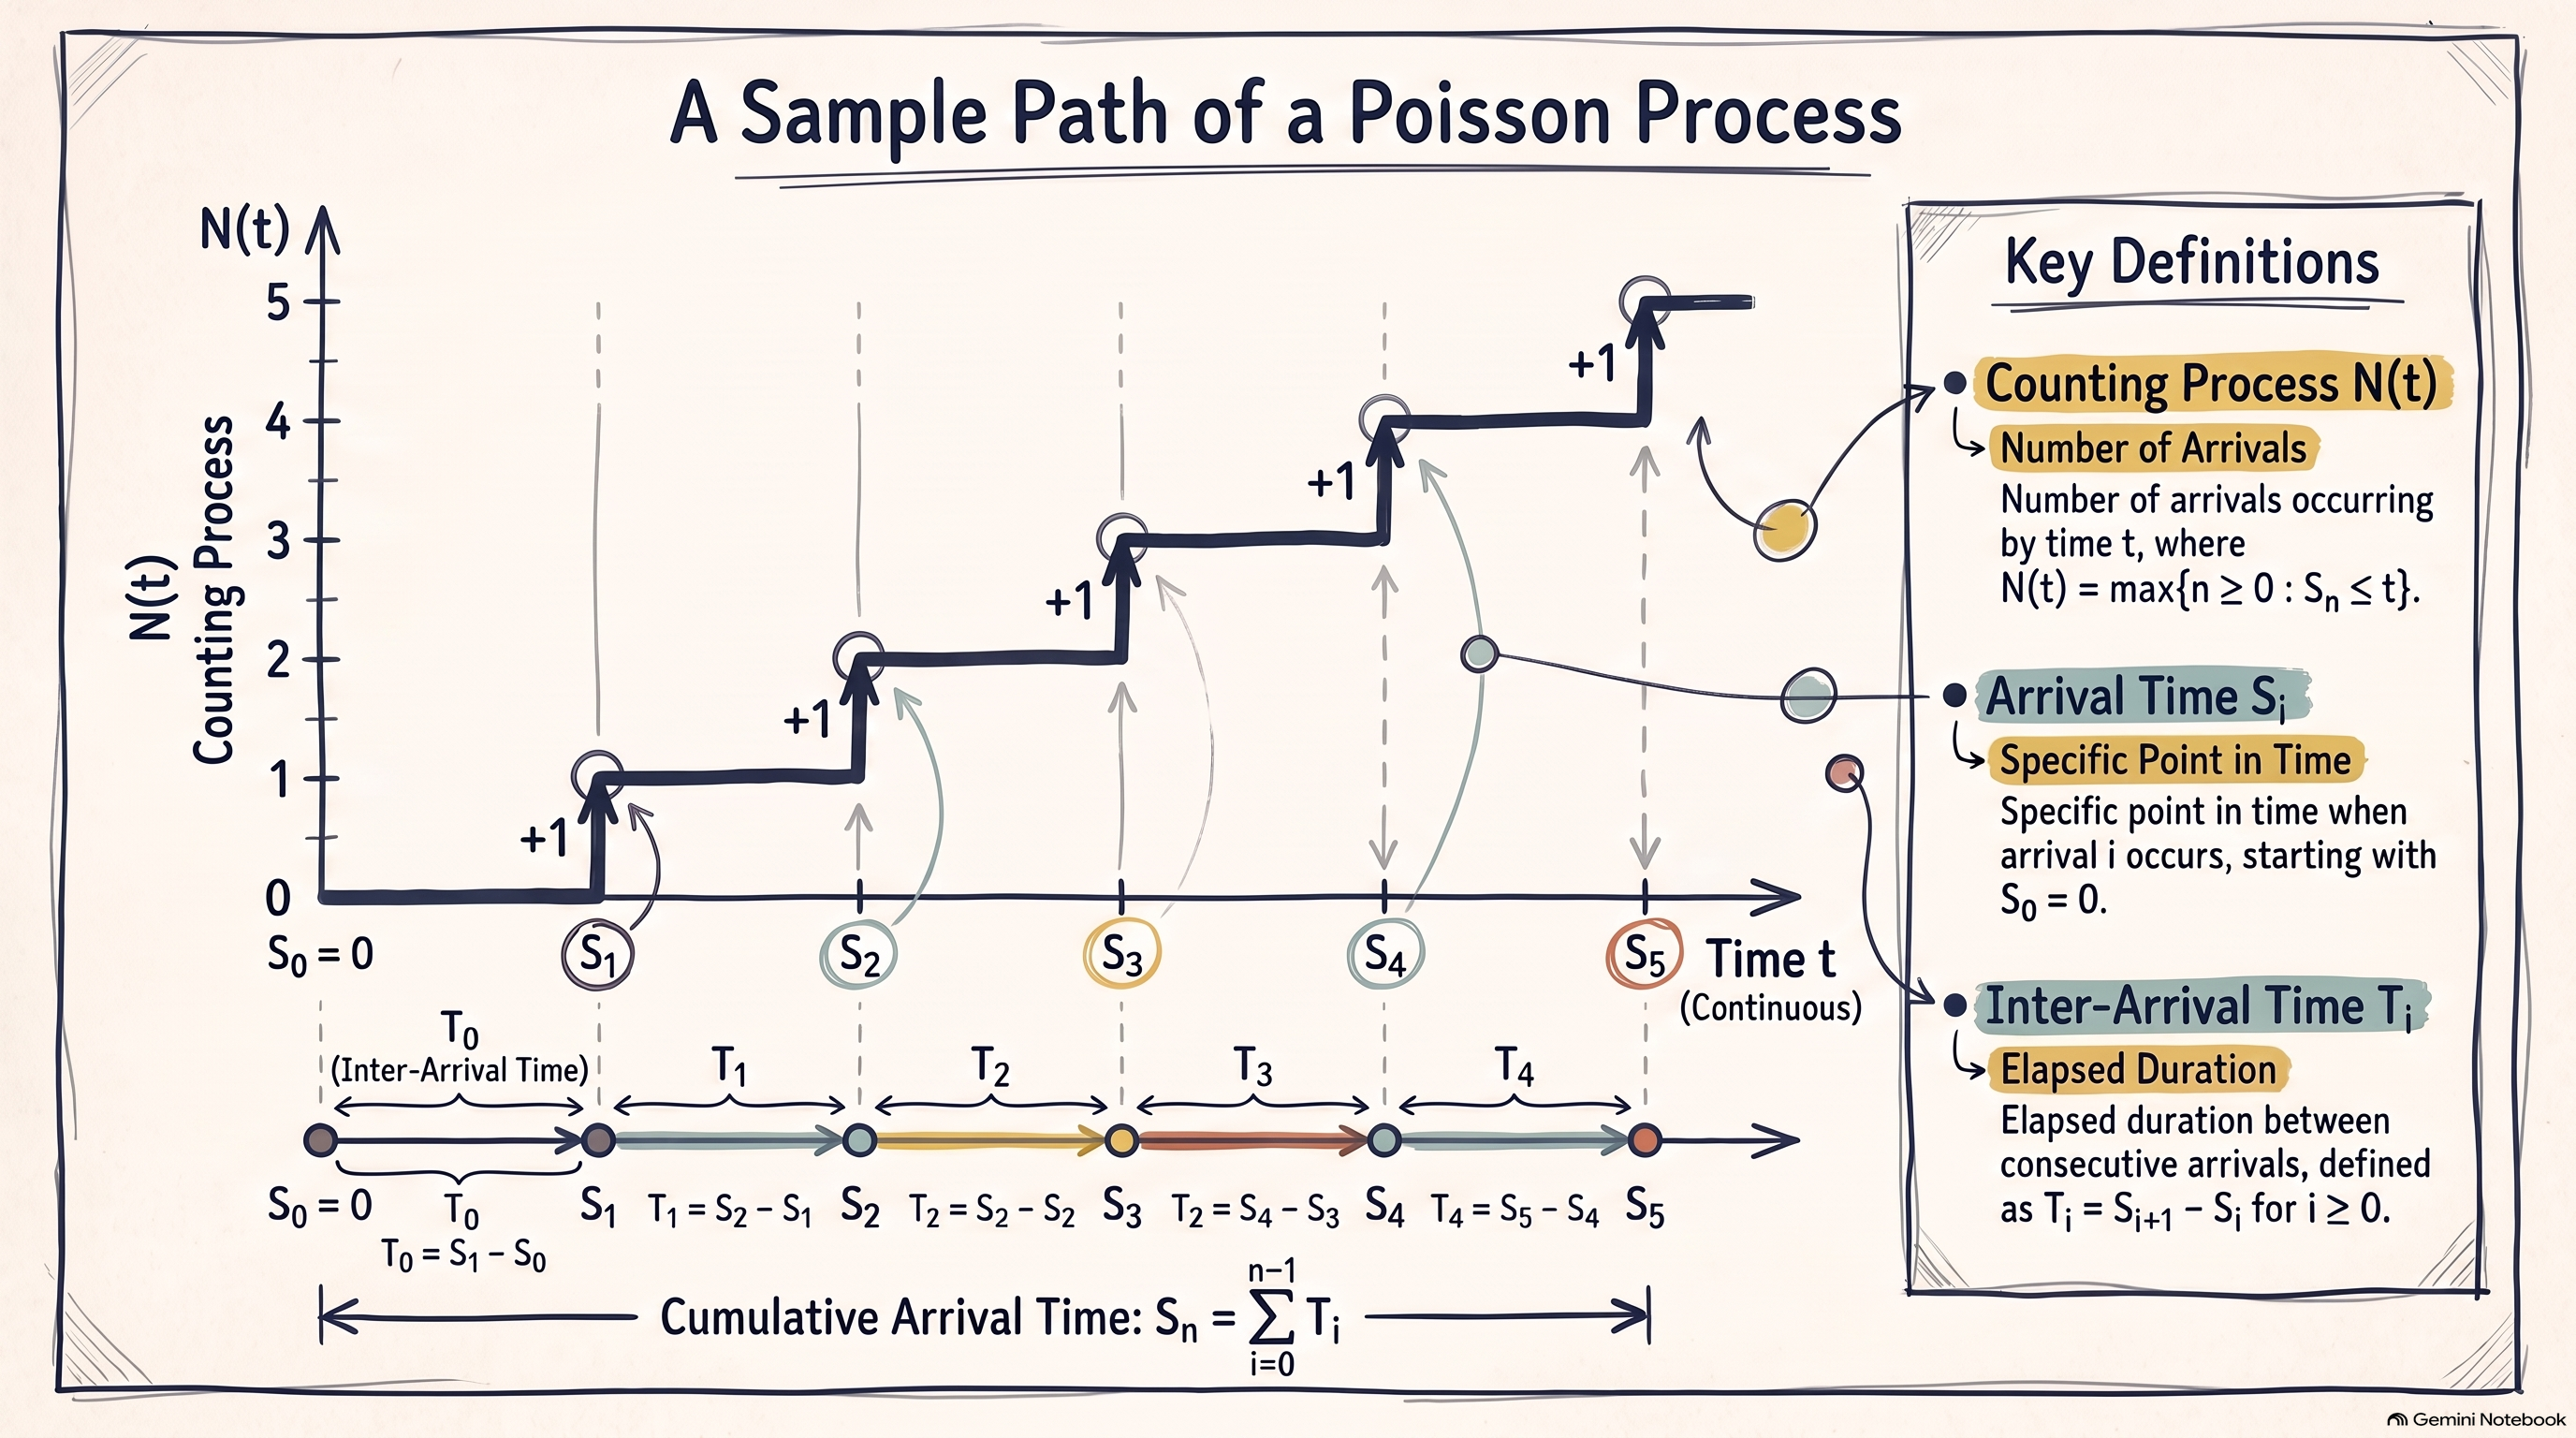
\includegraphics[width=0.75\linewidth,height=\textheight,keepaspectratio]{../figures/Poisson_Process_Sample_Path_Diagram.png}

}

\caption{Poisson Process Sample Path Diagram}

\end{figure}%
\end{frame}

\begin{frame}{Simulating a Sample Path}
\protect\phantomsection\label{simulating-a-sample-path}
A Poisson process can be simulated by generating successive
inter-arrival times and adding them to obtain the arrival times.

\begin{itemize}
\tightlist
\item
  Let \(T_i\) be the time between the \(i\)-th and \((i+1)\)-th
  arrivals, with \(T_0\) denoting the time until the first arrival.
\item
  Generate independent inter-arrival times from an exponential
  distribution with rate \(\lambda\).
\item
  Obtain the arrival times by taking cumulative sums.
\item
  The counting process \(N(t)\) increases by one at each arrival and
  remains constant between arrivals.
\end{itemize}
\end{frame}

\begin{frame}{Simulating a Sample Path}
\protect\phantomsection\label{simulating-a-sample-path-1}
\begin{figure}[H]

{\centering \pandocbounded{\includegraphics[keepaspectratio]{05_Slides_Poisson_Processes_files/figure-beamer/unnamed-chunk-1-1.pdf}}

}

\caption{A simulated sample path of a Poisson process}

\end{figure}%
\end{frame}

\begin{frame}[fragile]{Simulating a Sample Path: Set Up the Simulation}
\protect\phantomsection\label{simulating-a-sample-path-set-up-the-simulation}
\begin{Shaded}
\begin{Highlighting}[]
\FunctionTok{set.seed}\NormalTok{(}\DecValTok{888}\NormalTok{)}

\NormalTok{lambda }\OtherTok{\textless{}{-}} \DecValTok{12}
\NormalTok{T\_length }\OtherTok{\textless{}{-}} \DecValTok{1}

\CommentTok{\# Generate arrival times}
\NormalTok{arrival\_time }\OtherTok{\textless{}{-}} \FunctionTok{numeric}\NormalTok{()}
\NormalTok{last\_arrival }\OtherTok{\textless{}{-}} \DecValTok{0}
\end{Highlighting}
\end{Shaded}

\begin{itemize}
\tightlist
\item
  \texttt{lambda} is the arrival rate per unit time.
\item
  \texttt{T\_length} is the length of the observation interval.
\item
  \texttt{arrival\_time} stores the arrival times, while
  \texttt{last\_arrival} records the most recent arrival time.
\end{itemize}
\end{frame}

\begin{frame}[fragile]{Simulating a Sample Path: Generate Arrival Times}
\protect\phantomsection\label{simulating-a-sample-path-generate-arrival-times}
Generate independent exponential inter-arrival times and accumulate them
to obtain the arrival times.

\begin{Shaded}
\begin{Highlighting}[]
\ControlFlowTok{while}\NormalTok{ (last\_arrival }\SpecialCharTok{\textless{}}\NormalTok{ T\_length) \{}
\NormalTok{  inter\_arrival }\OtherTok{\textless{}{-}} \FunctionTok{rexp}\NormalTok{(}\DecValTok{1}\NormalTok{, }\AttributeTok{rate =}\NormalTok{ lambda)}
\NormalTok{  last\_arrival }\OtherTok{\textless{}{-}}\NormalTok{ last\_arrival }\SpecialCharTok{+}\NormalTok{ inter\_arrival}

  \ControlFlowTok{if}\NormalTok{ (last\_arrival }\SpecialCharTok{\textless{}}\NormalTok{ T\_length) \{}
\NormalTok{    arrival\_time }\OtherTok{\textless{}{-}} \FunctionTok{c}\NormalTok{(arrival\_time, last\_arrival)}
\NormalTok{  \}}
\NormalTok{\}}
\end{Highlighting}
\end{Shaded}

\begin{itemize}
\tightlist
\item
  Each inter-arrival time follows an exponential distribution with rate
  \texttt{lambda}.
\item
  Only arrivals occurring before \texttt{T\_length} are recorded.
\item
  The loop stops when the next arrival occurs at or beyond the
  observation horizon.
\end{itemize}
\end{frame}

\begin{frame}[fragile]{Simulating a Sample Path: Set Up the Plot}
\protect\phantomsection\label{simulating-a-sample-path-set-up-the-plot}
\begin{Shaded}
\begin{Highlighting}[]
\NormalTok{n }\OtherTok{\textless{}{-}} \FunctionTok{length}\NormalTok{(arrival\_time)}

\FunctionTok{plot}\NormalTok{(}\ConstantTok{NA}\NormalTok{, }\AttributeTok{xlim =} \FunctionTok{c}\NormalTok{(}\DecValTok{0}\NormalTok{, T\_length), }\AttributeTok{ylim =} \FunctionTok{c}\NormalTok{(}\DecValTok{0}\NormalTok{, n }\SpecialCharTok{+} \DecValTok{1}\NormalTok{),}
     \AttributeTok{xlab =} \StringTok{"Time t"}\NormalTok{, }\AttributeTok{ylab =} \StringTok{"N(t)"}\NormalTok{, }\AttributeTok{yaxt =} \StringTok{"n"}\NormalTok{)}

\FunctionTok{axis}\NormalTok{(}\DecValTok{2}\NormalTok{, }\AttributeTok{at =} \DecValTok{0}\SpecialCharTok{:}\NormalTok{n)}
\end{Highlighting}
\end{Shaded}

\begin{itemize}
\tightlist
\item
  Set the horizontal axis to the observation interval and the vertical
  axis to the possible count values.
\item
  \texttt{axis(2,\ at\ =\ 0:n)} displays integer values on the vertical
  axis.
\end{itemize}
\end{frame}

\begin{frame}[fragile]{Simulating a Sample Path: Draw the Jumps}
\protect\phantomsection\label{simulating-a-sample-path-draw-the-jumps}
\begin{Shaded}
\begin{Highlighting}[]
\NormalTok{previous\_time }\OtherTok{\textless{}{-}} \DecValTok{0}
\NormalTok{count }\OtherTok{\textless{}{-}} \DecValTok{0}

\ControlFlowTok{for}\NormalTok{ (t }\ControlFlowTok{in}\NormalTok{ arrival\_time) \{}
  \FunctionTok{points}\NormalTok{(previous\_time, count, }\AttributeTok{pch =} \DecValTok{16}\NormalTok{, }\AttributeTok{col =} \StringTok{"black"}\NormalTok{)}
  \FunctionTok{segments}\NormalTok{(previous\_time, count, t, count)}
\NormalTok{  previous\_time }\OtherTok{\textless{}{-}}\NormalTok{ t}
\NormalTok{  count }\OtherTok{\textless{}{-}}\NormalTok{ count }\SpecialCharTok{+} \DecValTok{1}
\NormalTok{\}}
\FunctionTok{points}\NormalTok{(previous\_time, count, }\AttributeTok{pch =} \DecValTok{16}\NormalTok{, }\AttributeTok{col =} \StringTok{"black"}\NormalTok{)}
\FunctionTok{segments}\NormalTok{(previous\_time, count, T\_length, count)}
\end{Highlighting}
\end{Shaded}

\begin{itemize}
\tightlist
\item
  The horizontal segments show that \(N(t)\) remains constant between
  arrivals.
\item
  At each arrival time, the process jumps upward by one.
\item
  The resulting sample path is a right-continuous step function.
\end{itemize}
\end{frame}

\begin{frame}{The Exponential Distribution}
\protect\phantomsection\label{the-exponential-distribution}
For a Poisson process with rate \(\lambda>0\), the event \(T_0>t\) means
that no arrivals occur during \([0,t]\).

Therefore,

\[
\begin{aligned}
\Pr(T_0>t)
&=\Pr(N(t)=0)\\
&=e^{-\lambda t},\qquad t\geq 0.
\end{aligned}
\]

Hence, \(T_0\) has an exponential distribution with rate \(\lambda\):

\[
T_0\sim\operatorname{Exp}(\lambda).
\]

Its density and mean are

\[
f_{T_0}(t)=\lambda e^{-\lambda t},
\quad t\geq 0,
\qquad
\operatorname{E}[T_0]=\frac{1}{\lambda}.
\]

The parameter \(\lambda\) is the expected number of arrivals per unit
time. Thus, the mean waiting time between arrivals is \(1/\lambda\).
\end{frame}

\begin{frame}{Independence of Inter-Arrival Times}
\protect\phantomsection\label{independence-of-inter-arrival-times}
The independent-increments property implies that the waiting time after
an arrival is independent of the history before that arrival.

For a Poisson process, the successive inter-arrival times are
independent and identically distributed:

\[
T_0,T_1,T_2,\ldots
\overset{\text{i.i.d.}}{\sim}
\operatorname{Exp}(\lambda).
\]

In particular, for \(s,t\geq 0\),

\[
\begin{aligned}
\Pr(T_0>s,T_1>t)
&=e^{-\lambda s}e^{-\lambda t}\\
&=\Pr(T_0>s)\Pr(T_1>t).
\end{aligned}
\]

This factorisation illustrates the independence of the first two
inter-arrival times. The same property holds for every finite collection
of successive inter-arrival times.
\end{frame}

\begin{frame}{Arrival Times and Their Distributions}
\protect\phantomsection\label{arrival-times-and-their-distributions}
The time of the \(n\)-th arrival is the sum of the first \(n\)
inter-arrival times:

\[
S_n=T_0+T_1+\cdots+T_{n-1}.
\]

Since the inter-arrival times are independent exponential random
variables with rate \(\lambda\),

\[
S_n\sim\operatorname{Gamma}(n,\text{ rate }\lambda),
\qquad n\geq 1.
\]

Its density is

\[
f_{S_n}(t)
=\frac{\lambda^n t^{n-1}e^{-\lambda t}}{(n-1)!},
\qquad t\geq 0.
\]

The event \(S_n\leq t\) is equivalent to having at least \(n\) arrivals
by time \(t\). Hence,

\[
\Pr(S_n\leq t)=\Pr(N(t)\geq n).
\]

Using the Poisson distribution,

\[
\Pr(S_n\leq t)
=1-\sum_{k=0}^{n-1}
\frac{(\lambda t)^k e^{-\lambda t}}{k!}.
\]

This connects the distribution of arrival times to the distribution of
the number of arrivals.
\end{frame}

\begin{frame}{Summary}
\protect\phantomsection\label{summary}
\begin{itemize}
\tightlist
\item
  Inter-arrival times are independent and exponentially distributed with
  rate \(\lambda\).
\item
  The mean inter-arrival time is \(1/\lambda\).
\item
  The \(n\)-th arrival time is the sum of \(n\) independent exponential
  random variables and has a gamma distribution.
\item
  The number of arrivals by time \(t\) has a Poisson distribution with
  mean \(\lambda t\).
\item
  These results allow us to simulate sample paths and calculate
  probabilities involving arrival times.
\end{itemize}
\end{frame}

\begin{frame}{Worked Example 6: Inter-Arrival Times}
\protect\phantomsection\label{worked-example-6-inter-arrival-times}
For a Poisson process with rate \(\lambda\), the inter-arrival times
\(\{T_i\}_{i\geq 0}\) are independent and identically distributed
exponential random variables with rate \(\lambda\).

Suppose events occur according to a Poisson process with rate
\(\lambda=3\) per hour.

\begin{enumerate}
\tightlist
\item
  State the distribution of the inter-arrival times.
\item
  Calculate the expected time between successive events.
\item
  Calculate the probability that the time between two successive events
  exceeds 30 minutes.
\end{enumerate}
\end{frame}

\begin{frame}{Solution: Worked Example 6}
\protect\phantomsection\label{solution-worked-example-6}
\end{frame}

\begin{frame}{Worked Example 7: Equipment Failures}
\protect\phantomsection\label{worked-example-7-equipment-failures}
In Worked Example 2, equipment malfunctions are modelled by a Poisson
process with rate \(1/8\) failures per hour.

Calculate the probability that the second failure occurs within one hour
of the first failure.
\end{frame}

\begin{frame}{Solution: Worked Example 7}
\protect\phantomsection\label{solution-worked-example-7}
\end{frame}

\begin{frame}{Worked Example 8: Insurance Claims}
\protect\phantomsection\label{worked-example-8-insurance-claims}
Insurance claims arrive according to a Poisson process with rate 5
claims per day.

\begin{enumerate}
\tightlist
\item
  Calculate the probability that at least two claims are reported on a
  given day.
\item
  Calculate the probability that another claim is reported within the
  next hour after a claim has just been reported.
\item
  Calculate the expected time until the next claim, given that no claims
  have been reported during the previous two days.
\end{enumerate}
\end{frame}

\begin{frame}{Solution: Worked Example 8}
\protect\phantomsection\label{solution-worked-example-8}
\end{frame}

\begin{frame}{Worked Example 9: Time Until the Second Arrival}
\protect\phantomsection\label{worked-example-9-time-until-the-second-arrival}
Customers arrive at a service centre according to a Poisson process with
rate 4 customers per hour.

\begin{enumerate}
\tightlist
\item
  State the distribution of the time until the second customer arrives.
\item
  Calculate the probability that the second customer arrives within 30
  minutes of the start of observation.
\item
  Calculate the expected time until the second customer arrives.
\end{enumerate}
\end{frame}

\begin{frame}{Solution: Worked Example 9}
\protect\phantomsection\label{solution-worked-example-9}
\end{frame}

\begin{frame}{Worked Example 10: Inter-Arrival Times and Arrival Times}
\protect\phantomsection\label{worked-example-10-inter-arrival-times-and-arrival-times}
Claims arrive according to a Poisson process with rate 2 claims per day.

\begin{enumerate}
\tightlist
\item
  Calculate the probability that the time between successive claims
  exceeds half a day.
\item
  Calculate the probability that the third claim arrives within two days
  of the start of observation.
\item
  Calculate the expected time until the third claim arrives.
\end{enumerate}
\end{frame}

\begin{frame}{Solution: Worked Example 10}
\protect\phantomsection\label{solution-worked-example-10}
The solution to this example will be provided later in the section on
\textbf{Conditional Distributions}.
\end{frame}

\section{Properties of the Poisson
Process}\label{properties-of-the-poisson-process}

\begin{frame}{Why Study the Properties?}
\protect\phantomsection\label{why-study-the-properties}
Poisson processes are useful for modelling events that occur randomly
over time, such as insurance claims, equipment failures, and customer
arrivals.

Their properties allow us to answer questions about event counts without
modelling every arrival time individually.

\begin{itemize}
\tightlist
\item
  \textbf{Independent increments:} Future counts over a new interval are
  independent of counts over earlier intervals.
\item
  \textbf{Stationary increments:} The distribution of the number of
  events depends on the interval length, not its starting time.
\item
  \textbf{Memorylessness:} The remaining waiting time has the same
  distribution as a fresh waiting time.
\item
  \textbf{Superposition:} Independent arrival streams can be combined
  into one Poisson process.
\item
  \textbf{Thinning:} A Poisson process can be divided into independent
  processes according to event types.
\end{itemize}
\end{frame}

\begin{frame}{Independent Increments}
\protect\phantomsection\label{independent-increments}
Suppose insurance claims follow a Poisson process with rate \(\lambda\)
claims per day.

The numbers of claims occurring during disjoint time intervals are
independent.

For \(0 \leq s < t \leq u < v\), the increments \(N(t)-N(s)\) and
\(N(v)-N(u)\) are independent.

For example, the number of claims on Monday is independent of the number
of claims on Tuesday.

More generally, counts over any collection of disjoint time intervals
are mutually independent.

This property allows us to calculate probabilities for different periods
separately.
\end{frame}

\begin{frame}{Stationary Increments}
\protect\phantomsection\label{stationary-increments}
The distribution of the number of events in an interval depends only on
its length.

For a Poisson process with rate \(\lambda\),

\[
N(t+h)-N(t)\sim \operatorname{Poisson}(\lambda h).
\]

Hence,

\[
\Pr(N(t+h)-N(t)=n)
=\frac{e^{-\lambda h}(\lambda h)^n}{n!},
\]

for \(n=0,1,2,\ldots\).

The expected number of events is \(\lambda h\), regardless of the
starting time \(t\).

For example, if claims arrive at a constant rate of 4 per day, the
number of claims in any one-day interval has a Poisson distribution with
mean 4.
\end{frame}

\begin{frame}{The Memoryless Property}
\protect\phantomsection\label{the-memoryless-property}
Suppose buses arrive according to a Poisson process with rate
\(\lambda\) per minute.

The waiting time \(X\) until the next bus has an exponential
distribution:

\[
X\sim\operatorname{Exponential}(\lambda).
\]

Its survival function is \(\Pr(X>t)=e^{-\lambda t}\).

The memoryless property states that, for \(s,t\geq 0\),

\[
\Pr(X>s+t\mid X>s)=\Pr(X>t).
\]

Therefore, conditional on having waited \(s\) minutes without a bus
arriving, the remaining waiting time has the same exponential
distribution as the original waiting time.

The process does not become more or less likely to produce an arrival
simply because no arrival has occurred recently.
\end{frame}

\begin{frame}{Why Memorylessness Matters}
\protect\phantomsection\label{why-memorylessness-matters}
Suppose buses arrive, on average, once every 30 minutes. The
interarrival times are exponentially distributed with rate
\(\lambda=1/30\) per minute.

If no bus has arrived during the first 10 minutes, the probability of
waiting at least another 20 minutes is

\[
\begin{aligned}
\Pr(X>30\mid X>10)
&=\frac{\Pr(X>30)}{\Pr(X>10)}\\
&=\frac{e^{-30/30}}{e^{-10/30}}\\
&=e^{-20/30}.
\end{aligned}
\]

This is exactly the probability that a new waiting time exceeds 20
minutes.

The memoryless property is specific to the exponential distribution
among continuous distributions. It is also a key reason exponential
interarrival times are used in Poisson process models.
\end{frame}

\begin{frame}{Worked Example 11: Time Spent at a Dentist's Office}
\protect\phantomsection\label{worked-example-11-time-spent-at-a-dentists-office}
Assume that the amount of time a patient spends in a dentist's office
follows an exponential distribution with a mean of 40 minutes.

\begin{enumerate}
\item
  Calculate the probability that a patient spends more than 60 minutes
  in the dentist's office.
\item
  Calculate the probability that a patient spends more than 60 minutes
  in the dentist's office, given that she has already spent 40 minutes
  there.
\end{enumerate}
\end{frame}

\begin{frame}{Solution: Worked Example 11}
\protect\phantomsection\label{solution-worked-example-11}
\end{frame}

\begin{frame}{Superposition of Independent Poisson Processes}
\protect\phantomsection\label{superposition-of-independent-poisson-processes}
Consider several independent sources of arrivals, each modelled by a
Poisson process.

Examples include claims from different insurance portfolios, customer
arrivals at different entrances, or failures from different types of
equipment.

Let \(N_1(t),\ldots,N_k(t)\) be independent Poisson processes with rates
\(\lambda_1,\ldots,\lambda_k\).

The combined process is

\[
N(t)=\sum_{i=1}^{k}N_i(t).
\]
\end{frame}

\begin{frame}{Superposition: Combined Arrival Rate}
\protect\phantomsection\label{superposition-combined-arrival-rate}
By the superposition property, \(N(t)\) is a Poisson process with rate

\[
\lambda=\sum_{i=1}^{k}\lambda_i.
\]

For any interval of length \(h\),

\[
N(t+h)-N(t)\sim
\operatorname{Poisson}\left(h\sum_{i=1}^{k}\lambda_i\right).
\]

The combined arrival rate is the sum of the individual rates. This
allows us to model arrivals from several independent sources as a single
Poisson process.
\end{frame}

\begin{frame}{Superposition Roadmap}
\protect\phantomsection\label{superposition-roadmap}
\begin{figure}[H]

{\centering 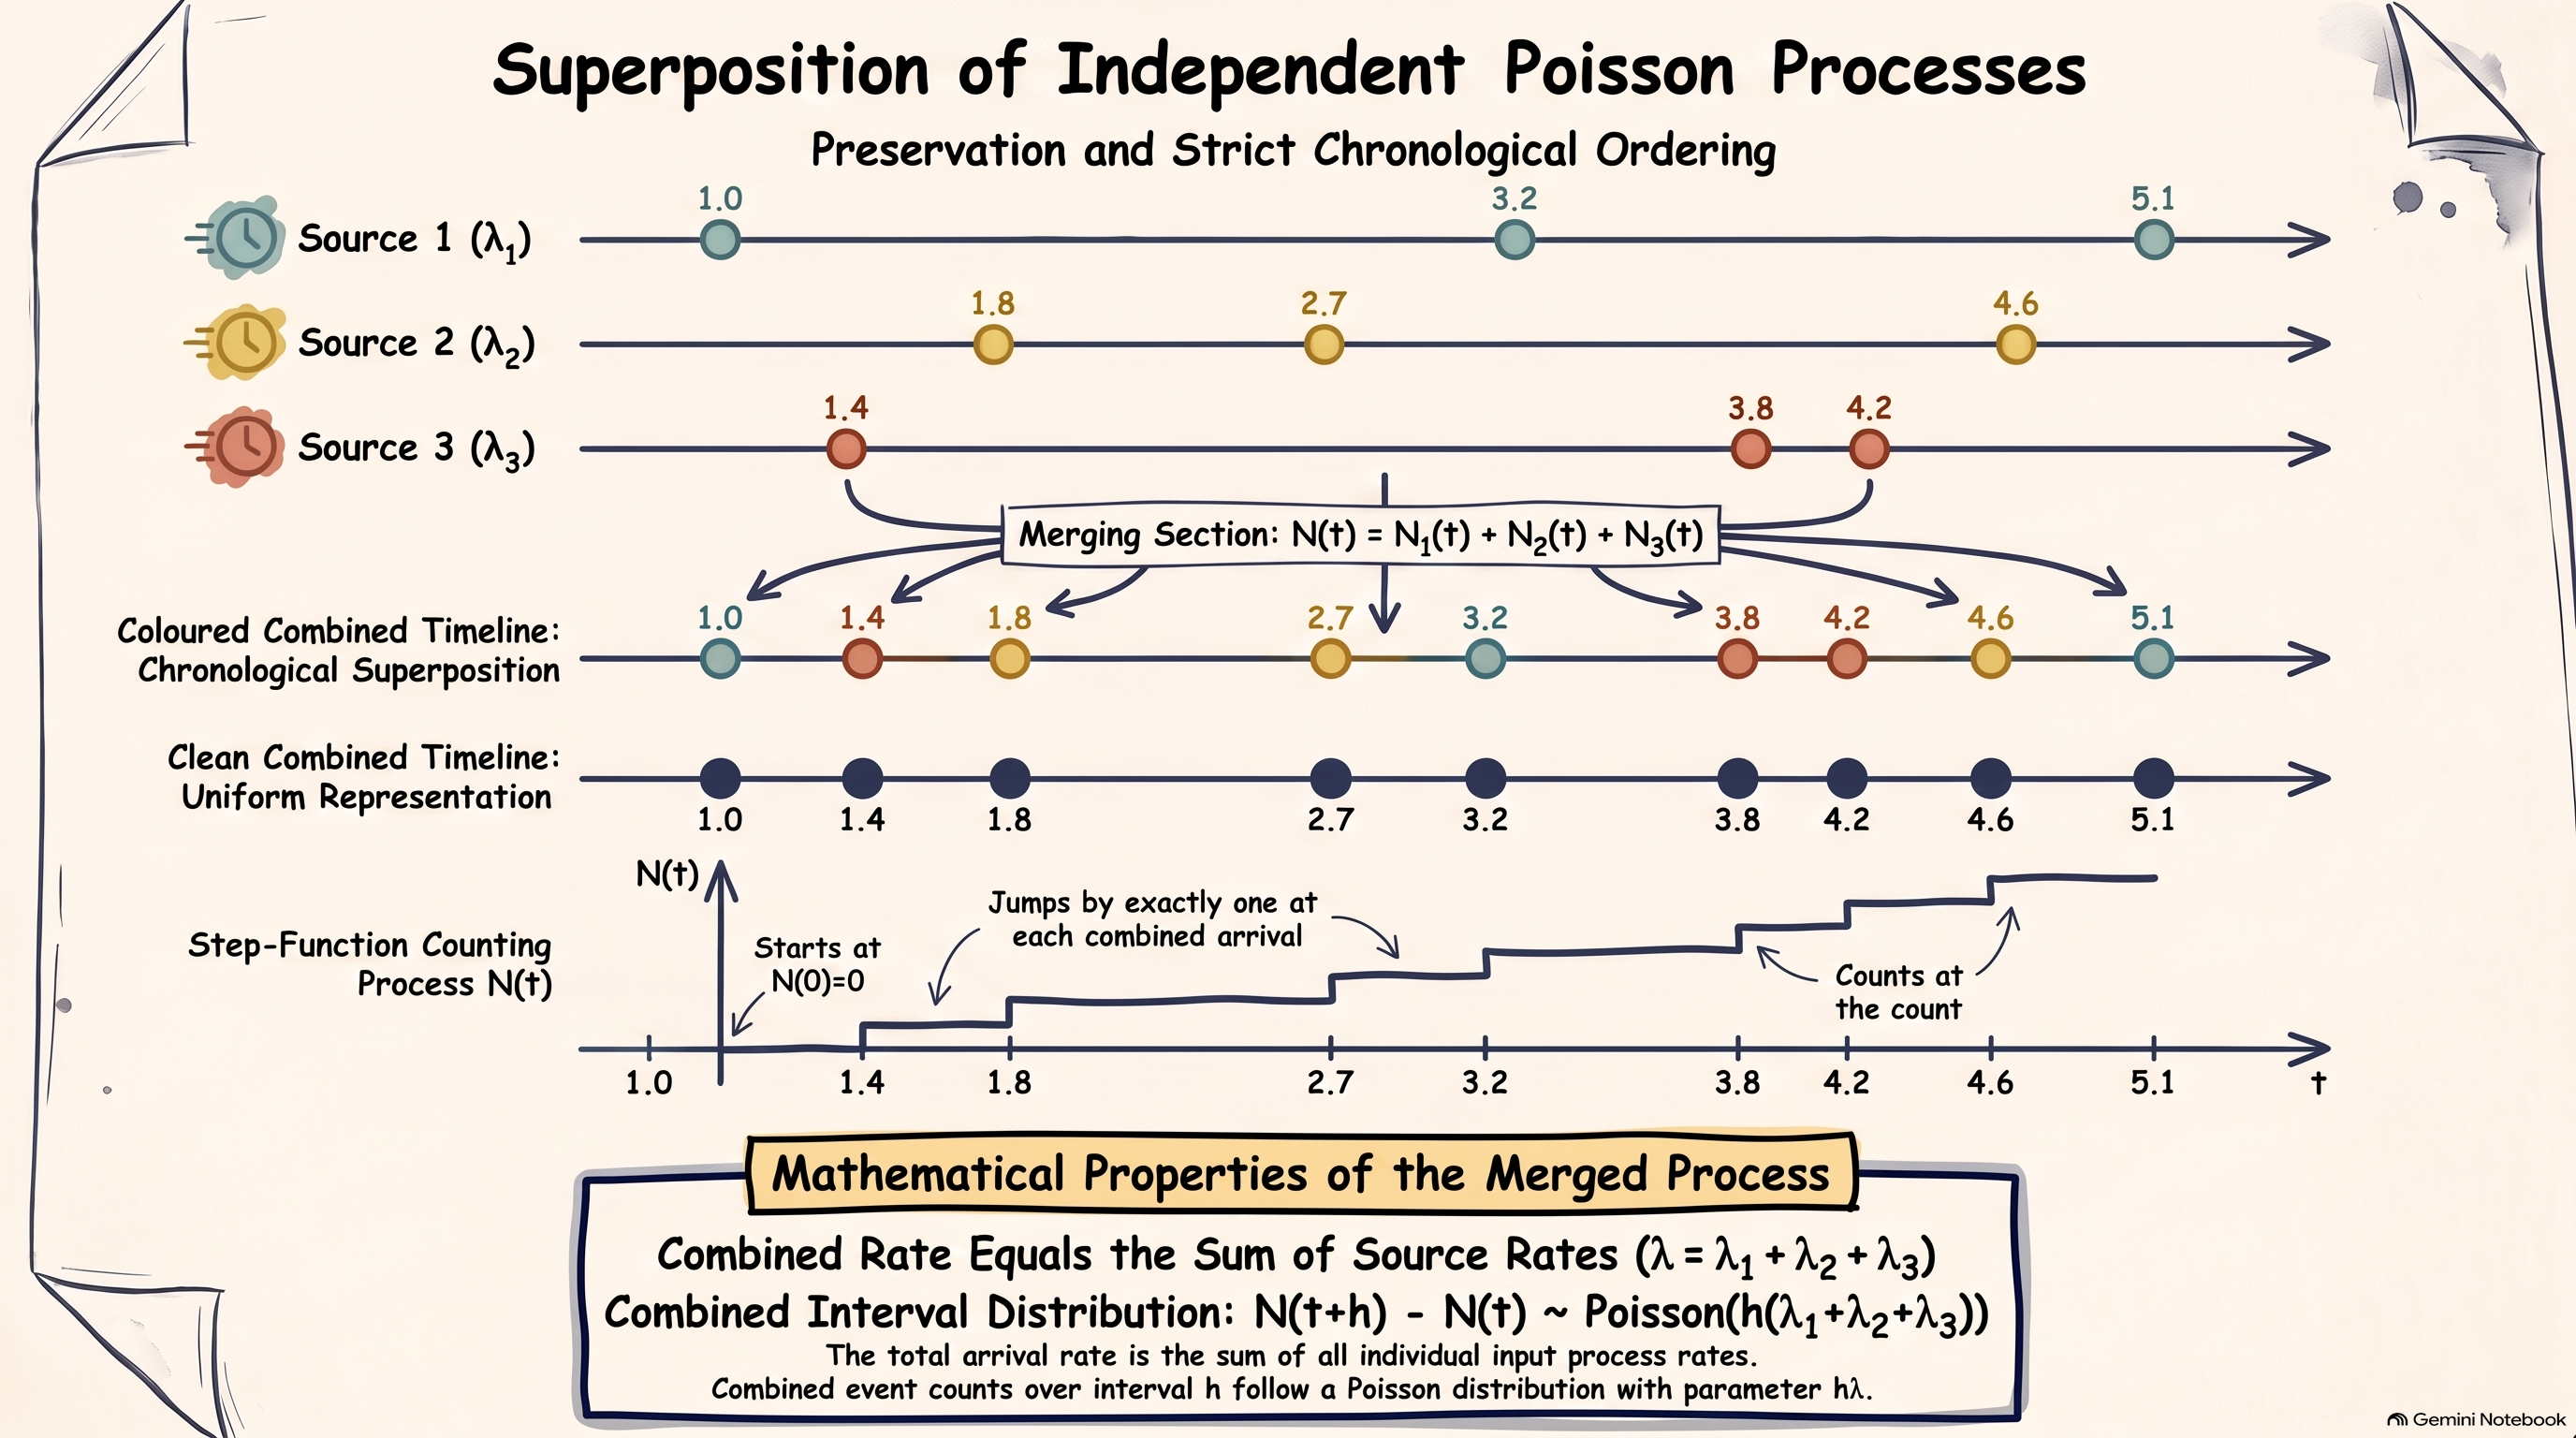
\includegraphics[width=0.75\linewidth,height=\textheight,keepaspectratio]{../figures/Superposition_of_Independent_Poisson_Processes.png}

}

\caption{Superposition of Independent Poisson Processes}

\end{figure}%
\end{frame}

\begin{frame}{Identifying the Source of an Arrival}
\protect\phantomsection\label{identifying-the-source-of-an-arrival}
Suppose independent Poisson processes with rates
\(\lambda_1,\ldots,\lambda_k\) are combined into a single process with
rate \(\lambda=\sum_{i=1}^k\lambda_i\).

Given an arrival in the combined process, the probability that it comes
from source \(i\) is

\[
p_i=\frac{\lambda_i}{\lambda}.
\]

The source of each arrival can therefore be viewed as an independent
categorical outcome with probabilities \(p_1,\ldots,p_k\).

For two sources with rates 2 and 6 per day, the combined rate is 8 per
day. Each arrival has probability \(2/8=1/4\) of coming from the first
source and probability \(6/8=3/4\) of coming from the second.
\end{frame}

\begin{frame}{Identifying the Source of an Arrival}
\protect\phantomsection\label{identifying-the-source-of-an-arrival-1}
\begin{block}{Note}
The source of each arrival can be modelled by a discrete random variable $X$, where $X=i$ indicates that the arrival comes from source $i$. Its probability mass function is

$$
P(X=i)=p_i,\qquad i=1,\ldots,k.
$$
\end{block}
\end{frame}

\begin{frame}{Splitting and Thinning of a Poisson Process}
\protect\phantomsection\label{splitting-and-thinning-of-a-poisson-process}
Suppose arrivals follow a Poisson process with rate \(\lambda\). Each
arrival is independently assigned to one of \(k\) types, with
probabilities \(p_1,\ldots,p_k\), where \(\sum_{i=1}^k p_i=1\).

Let \(N_i(t)\) count the type \(i\) arrivals by time \(t\).

The splitting (or sampling) property states that
\(N_1(t),\ldots,N_k(t)\) are independent Poisson processes with
respective rates

\[
\lambda_i=p_i\lambda,\qquad i=1,\ldots,k.
\]

Each resulting process is called a \emph{thinned Poisson process}.

The rate of each type is the original rate multiplied by the probability
of belonging to that type.
\end{frame}

\begin{frame}{Splitting and Thinning Roadmap}
\protect\phantomsection\label{splitting-and-thinning-roadmap}
\begin{figure}[H]

{\centering 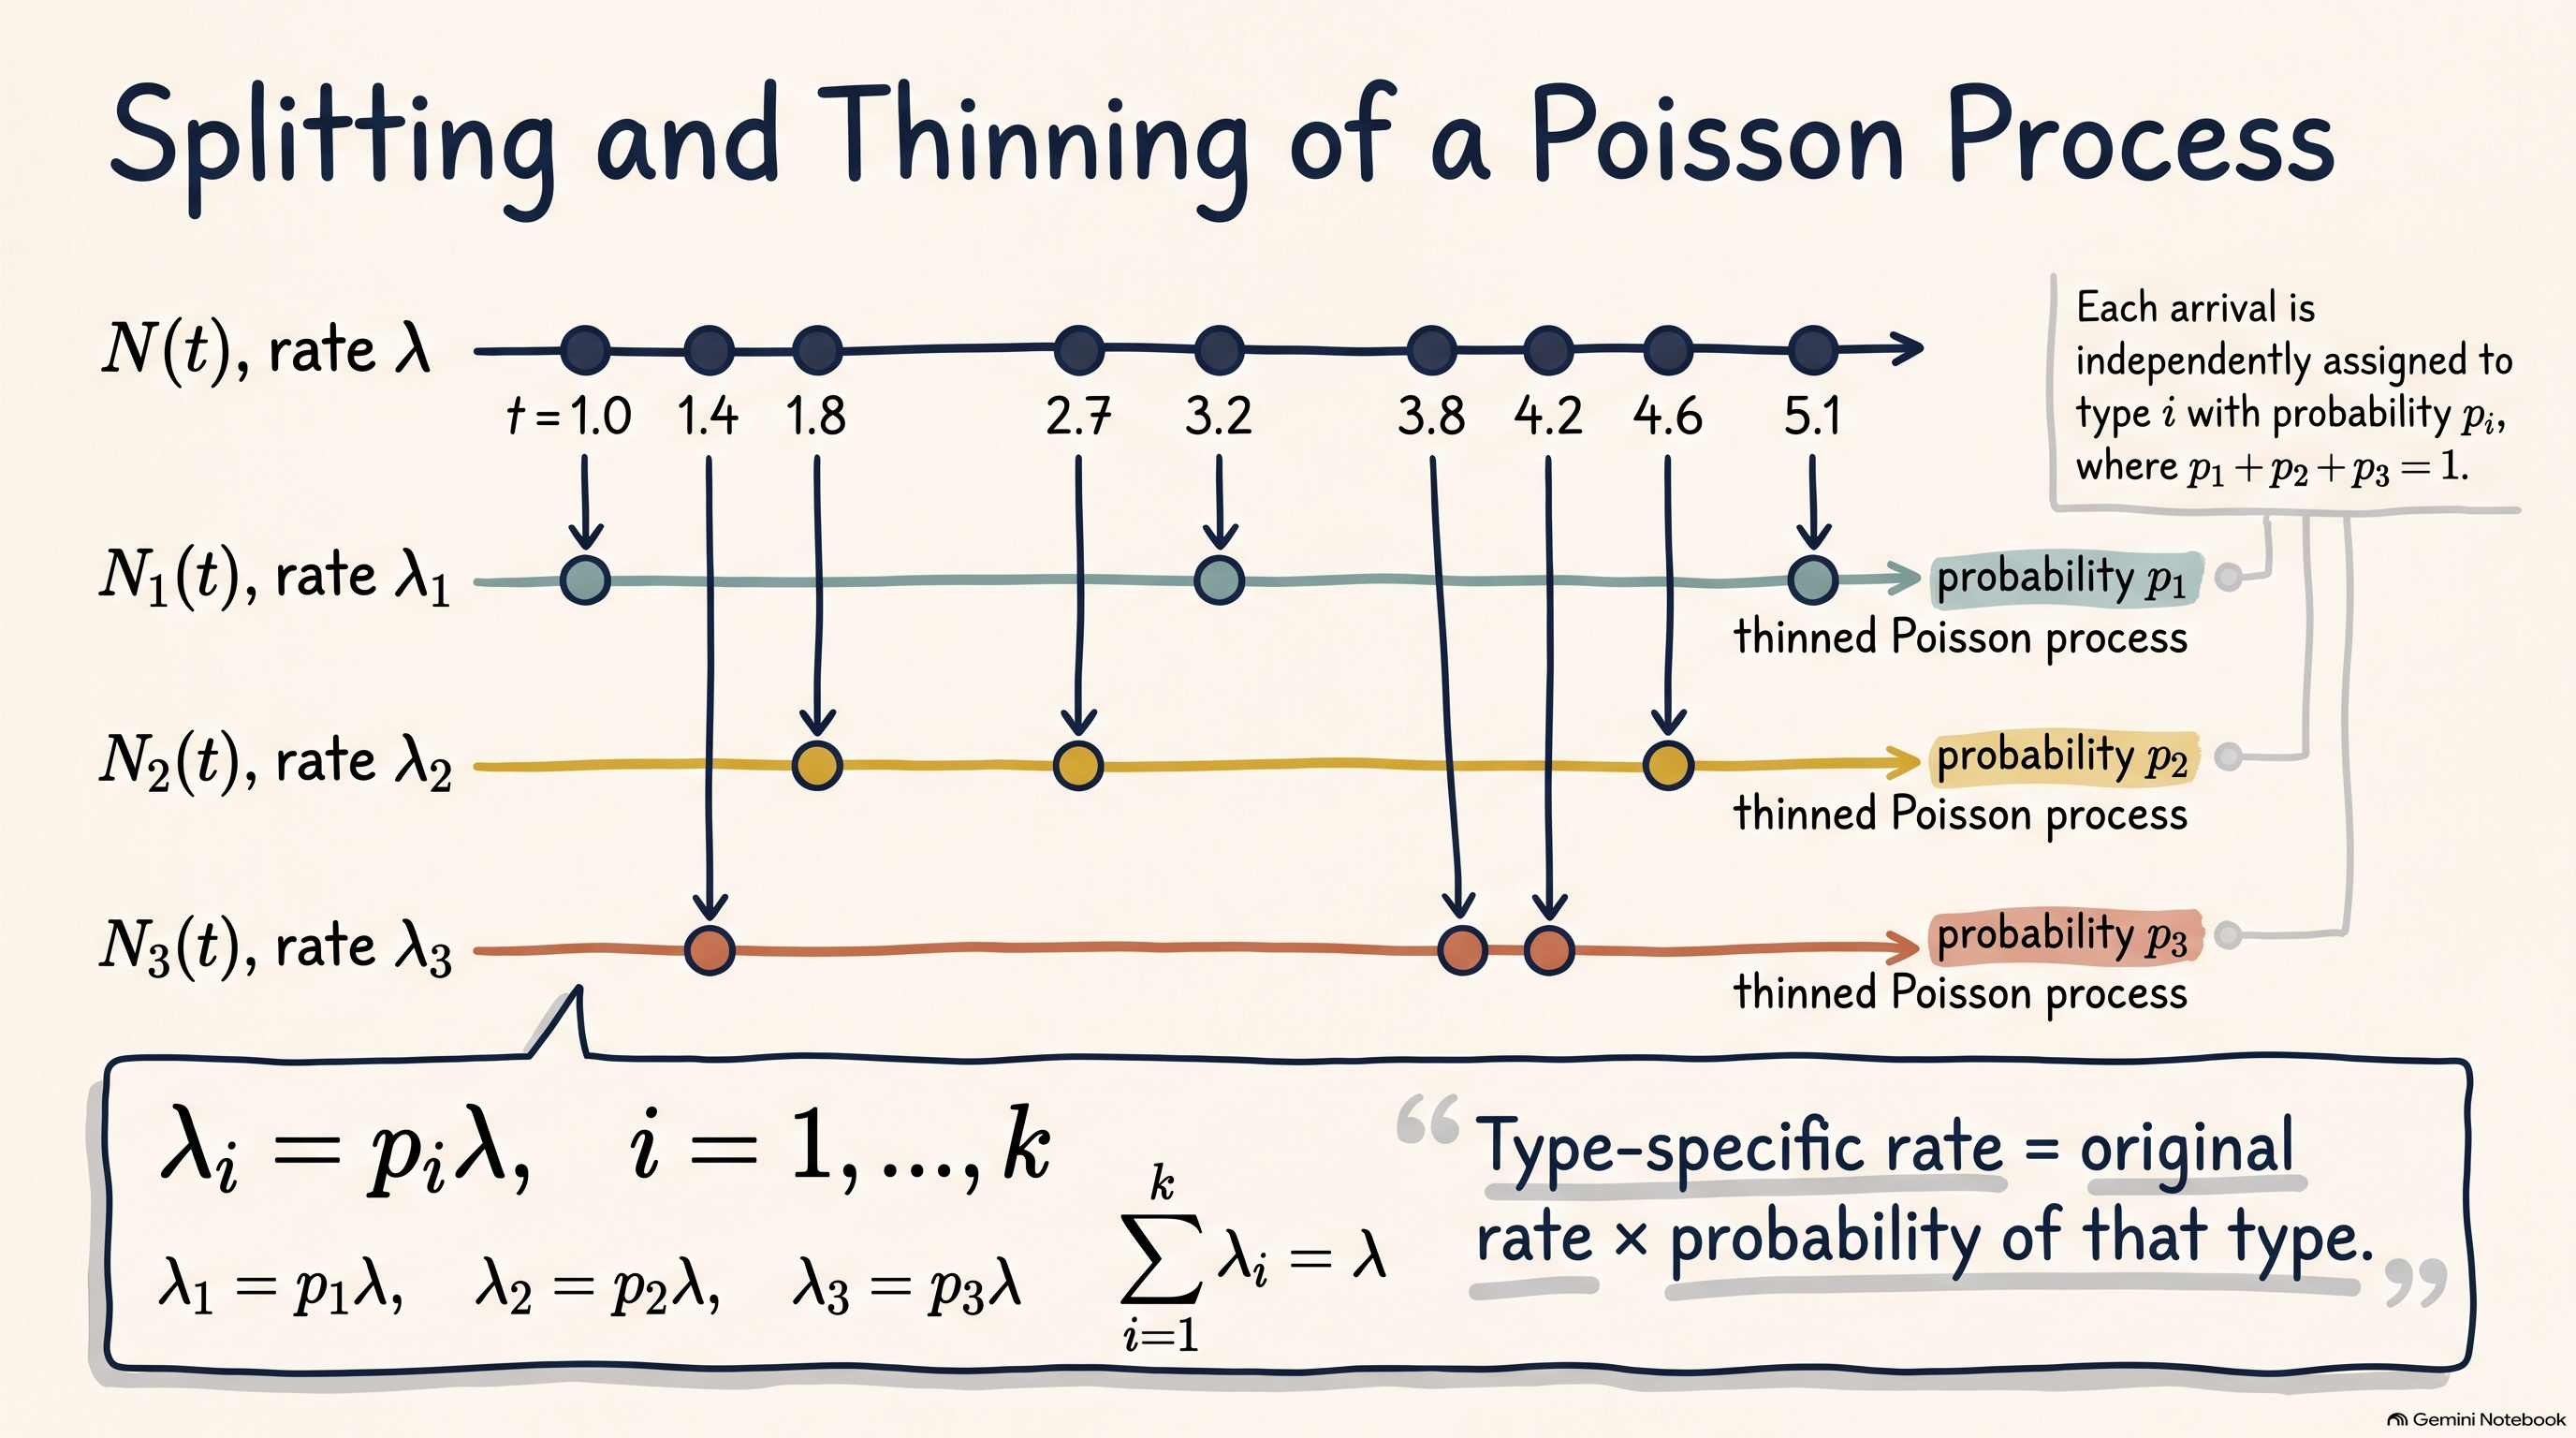
\includegraphics[width=0.75\linewidth,height=\textheight,keepaspectratio]{../figures/Splitting_and_Thinning_Poisson_Process.png}

}

\caption{Splitting and Thinning Poisson Process}

\end{figure}%
\end{frame}

\begin{frame}{Why Thinning Matters in Insurance}
\protect\phantomsection\label{why-thinning-matters-in-insurance}
An insurer may be interested in only some of its claims, such as claims
exceeding a specified threshold.

Suppose claims arrive at rate \(\lambda\) and each claim independently
meets the threshold with probability \(p\).

The claims meeting the threshold form a Poisson process with rate

\[
\lambda_{\text{selected}}=p\lambda.
\]

This allows us to model large claims directly without first modelling
all claims and then identifying which ones are large.

For independent portfolios, thinning can be applied to each portfolio
separately, and superposition can then combine the selected claims.
\end{frame}

\begin{frame}{Worked Example 12: Claims Above a Threshold}
\protect\phantomsection\label{worked-example-12-claims-above-a-threshold}
An insurer has two independent portfolios, A and B.

\begin{itemize}
\tightlist
\item
  Claims from A arrive at rate 4 per day. Each claim has probability
  \(2/5\) of being at least 5,000 THB.
\item
  Claims from B arrive at rate 6 per day. Each claim has probability
  \(1/3\) of being at least 5,000 THB.
\end{itemize}

Calculate the expected number of claims of at least 5,000 THB during the
next day.
\end{frame}

\begin{frame}{Solution: Worked Example 12}
\protect\phantomsection\label{solution-worked-example-12}
\end{frame}

\begin{frame}{Worked Example 13: Claims from Two Groups}
\protect\phantomsection\label{worked-example-13-claims-from-two-groups}
Claims from male policyholders and female policyholders arrive
independently according to Poisson processes with rates 2 and 6 per day,
respectively.

\begin{enumerate}
\tightlist
\item
  Calculate the probabilities of no claims and at least two claims
  during a given week.
\item
  Calculate the probability that four claims from female policyholders
  occur before the second claim from a male policyholder.
\end{enumerate}
\end{frame}

\begin{frame}{Solution: Worked Example 13}
\protect\phantomsection\label{solution-worked-example-13}
\end{frame}

\begin{frame}{Summary}
\protect\phantomsection\label{summary-1}
The properties of a Poisson process provide several useful modelling
tools.

\begin{itemize}
\tightlist
\item
  Independent and stationary increments describe counts over disjoint
  intervals.
\item
  The memoryless property explains why exponential waiting times are
  appropriate for Poisson arrivals.
\item
  Superposition combines independent arrival streams by adding their
  rates.
\item
  Thinning selects events by independent classification and multiplies
  the rate by the selection probability.
\end{itemize}

Together, these properties simplify calculations involving arrivals from
multiple sources, selected event types, and waiting times.
\end{frame}




\end{document}
